\section{Performance of Path Following}

Due to delays in the project converting the go-kart to a point where it could be interfaced with the laptop the algorithm was never tested on the kart. To allow for some basic testing a simple GUI output was instead added to the program. This mapped the absolute location of the kart and the chessboard as well as the path they had taken. It also highlighted the point which the kart was currently driving towards. Fake input from the steering and speed sensors were created giving the kart a constant speed and a maximum turn rate of 30 degrees per second. This system is shown in Figure~\ref{tracking}. This interface allowed the system to be debugged and tested though was fairly limited in comparison to the actual go-kart. Its largest problem was that as the system believed that it was moving forward and turning it saw a stationary marker in front of it as moving to maintain the same relative position. This meant that testing the system's ability to follow patterns laid out by the marker was seriously hindered.

\begin{figure}[ht]
	\begin{center}
		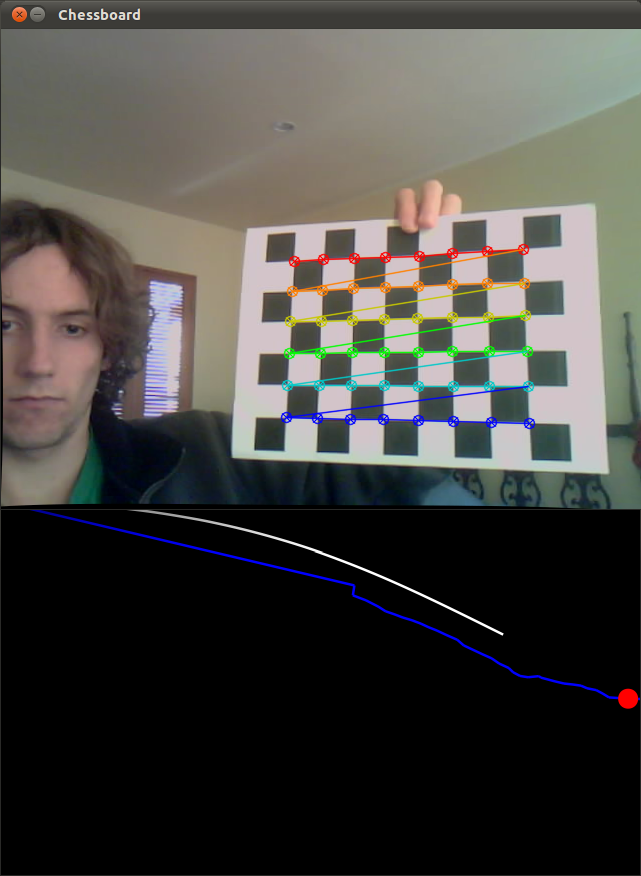
\includegraphics[width=0.3\textwidth]{tracking}
	\end{center}
	\caption{Path finding GUI using chessboard detection. The path of the kart is shown in white, blue for the chessboard and the red dot is the current point the kart is driving towards}
	\label{tracking}
\end{figure}